\chapter{\texorpdfstring{Petri Nets}{Petri Nets}}
\label{ch:04}
\lecturemeta{Lezione 04 \quad\textbullet\quad 2026-07-03 \quad\textbullet\quad Roberto Bruni}{Weske, \emph{Business Process Management}, Ch.4.4}

Nella lezione precedente (\hyperref[ch:03]{03 — Visual Notation}) abbiamo scoperto un problema serio: un grafo fatto di soli nodi e frecce è \textbf{ambiguo}. Guardando le frecce non riusciamo a dire se, dopo un certo passo, due attività vanno svolte \emph{entrambe} (in parallelo) oppure se ne va scelta \emph{una sola}. Avevamo tamponato il problema aggiungendo dei gateway \texttt{+} e \texttt{✕}, ma quei simboli erano solo una convenzione grafica, senza una vera regola matematica dietro.

I \textbf{Petri net} risolvono il problema alla radice. Invece di aggiungere decorazioni a un grafo, cambiano proprio il \emph{tipo} di grafo: ne usano uno in cui la distinzione tra "fare entrambi" e "scegliere uno" \textbf{emerge automaticamente dalla struttura}, senza bisogno di simboli speciali. In più forniscono una \textbf{semantica formale}, cioè una regola precisa e meccanica che dice, passo dopo passo, come il processo evolve. Questo ha due conseguenze importanti:

\begin{itemize}
\item \textbf{Formale} significa che il comportamento di ogni istanza del processo diventa \emph{non ambiguo}: dato lo stato attuale, le mosse possibili sono determinate da una regola, non dall'interpretazione di chi legge.
\item \textbf{Astratto} significa che ci concentriamo solo sulla logica del processo, ignorando l'ambiente di esecuzione (chi esegue, su quale macchina, con quali dati concreti). È il principio di \emph{separation of concerns}: un problema alla volta.
\end{itemize}

Furono introdotti da \textbf{Carl Adam Petri} (1926–2010) nella sua tesi di dottorato del \textbf{1962}. Il loro successo, che dagli anni '60 li ha portati fino a essere applicati oggi in moltissimi campi, si deve a una rappresentazione grafica e concettuale tanto semplice quanto potente. Per noi saranno la \textbf{base semantica} su cui costruiremo tutta l'analisi dei processi nel resto del corso.

\section{\texorpdfstring{Gli elementi di base}{Gli elementi di base}}

Un Petri net è un grafo di tipo particolare, detto \textbf{bipartito}: ha due tipi di nodi diversi che si alternano sempre, e non si collegano mai due nodi dello stesso tipo. I due tipi di nodo sono i \textbf{place} e le \textbf{transition}; sopra di essi si muovono i \textbf{token}. Prima di dare le definizioni precise, conviene capire \emph{a cosa servono} con un'immagine mentale.

Pensiamo a un processo come a qualcosa che scorre attraverso una serie di \textbf{condizioni} (stati in cui il processo si può trovare) e di \textbf{eventi} (cose che accadono e fanno passare il processo da una condizione all'altra). Nei Petri net:

\begin{itemize}
\item le \textbf{condizioni} sono i \textbf{place} (i cerchi): rappresentano \emph{dove si trova} il processo, cioè uno stato in attesa che qualcosa accada;
\item gli \textbf{eventi} sono le \textbf{transition} (i quadrati): rappresentano \emph{qualcosa che succede}, un'azione che trasforma lo stato;
\item ciò che effettivamente \emph{scorre} e segnala in quale condizione siamo sono i \textbf{token} (i pallini dentro i cerchi).
\end{itemize}

\begin{boxdefinition}{Transition (i quadrati)}
Una \textbf{transition} rappresenta \emph{qualcosa che accade}: un'operazione, un calcolo, una valutazione, una trasformazione, una spedizione, un task, un'attività, una decisione. È la parte "attiva" della rete: quando una transition scatta, lo stato del processo cambia.
\end{boxdefinition}

\begin{boxdefinition}{Place (i cerchi)}
Un \textbf{place} rappresenta una \emph{condizione} o uno \emph{stato} in cui il processo si può trovare: uno stato di attesa, un medium, un buffer, una condizione da soddisfare, un deposito di risorse, un tipo, una locazione di memoria. È la parte "passiva": da solo non fa nulla, ma \textbf{contiene i token} e così registra la situazione corrente.
\end{boxdefinition}

\begin{boxdefinition}{Token (i pallini)}
Un \textbf{token} è ciò che \emph{popola} un place e indica che quella condizione è soddisfatta. A seconda di cosa stiamo modellando, un token può rappresentare un oggetto fisico, un dato, un record, una risorsa disponibile, una marca di attivazione, un messaggio, un documento, un \textbf{caso} in lavorazione, un valore. La distribuzione dei token nei place (la \textbf{marcatura}) è lo \emph{stato} del sistema in un dato istante.
\end{boxdefinition}

\begin{boxtip}{L'analogia utile}
Immaginiamo un ambulatorio: un \textbf{place} è la sala d'attesa (una condizione: "paziente in attesa di visita"), una \textbf{transition} è la visita medica (l'evento che accade), il \textbf{token} è il paziente che occupa la sala. Finché c'è un paziente in sala (token nel place), la visita \emph{può} avvenire; quando avviene (la transition scatta), il paziente lascia la sala e passa alla condizione successiva.
\end{boxtip}

\subsection{\texorpdfstring{Gli archi: come si collegano place e transition}{Gli archi: come si collegano place e transition}}

I nodi sono collegati da \textbf{archi} orientati. La regola fondamentale è che un arco unisce \textbf{sempre} un place a una transition o viceversa, \textbf{mai} due nodi dello stesso tipo. Questa alternanza obbligata è ciò che rende la rete bipartita, ed è anche ciò che dà significato agli archi: un arco descrive sempre un rapporto tra una \emph{condizione} e un \emph{evento}.

\begin{boxdefinition}{Arc}
Un \textbf{arc} rappresenta una \textbf{dipendenza}, e ha due sole forme possibili:

\begin{itemize}
\item \textbf{da un place a una transition}:
\end{itemize}

\begin{itemize}
\item \textbf{da una transition a un place}:
\end{itemize}
\end{boxdefinition}

\begin{boxwarning}{Archi vietati}
Non esistono archi \textbf{place $\rightarrow$ place} né \textbf{transition $\rightarrow$ transition}. Due condizioni non si collegano direttamente (serve sempre un evento in mezzo), e due eventi nemmeno (serve sempre una condizione in mezzo). Se disegnando una rete vi trovate un arco tra due cerchi o tra due quadrati, la rete \textbf{non è valida}.
\end{boxwarning}

\begin{center}
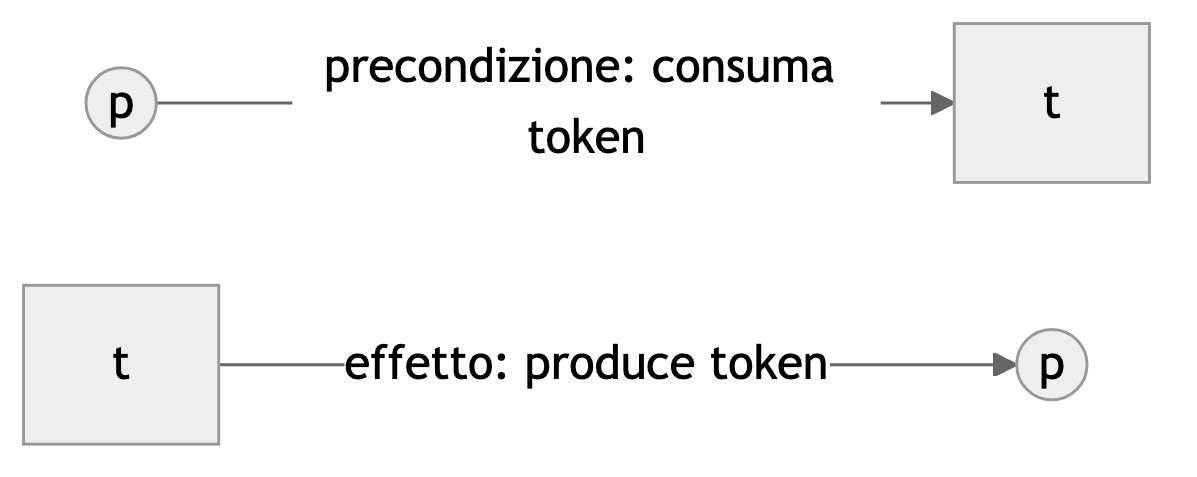
\includegraphics[width=0.74\linewidth,height=0.32\textheight,keepaspectratio]{images/mermaid/04_1.png}
\end{center}

\emph{Fig. — A sinistra un place che fa da precondizione a una transition; a destra una transition che produce un token in un place.}

\section{\texorpdfstring{La definizione formale}{La definizione formale}}

Ora che l'intuizione è chiara, possiamo scrivere la definizione precisa. Una rete è completamente descritta dicendo quali sono i suoi place, quali le sue transition, come sono collegati e da quale configurazione di token si parte.

\begin{boxdefinition}{Petri net}
Una \textbf{Petri net} è una tupla: \((P, T, F, M_0)\) dove:

\begin{itemize}
\item $P$ è un insieme \textbf{finito} di \textbf{place};
\item $T$ è un insieme \textbf{finito} di \textbf{transition}, disgiunto dai place:
\item $F \subseteq (P \times T) \cup (T \times P)$ è la \textbf{flow relation}, cioè l'insieme degli archi: ogni arco è una coppia place–transition o transition–place, mai place–place o transition–transition (è qui che si formalizza la bipartizione);
\item $M_0$ è l'\textbf{initial marking}: la configurazione iniziale dei token, cioè quanti token stanno in ciascun place all'inizio.
\end{itemize}
\end{boxdefinition}

Una volta fissata la struttura, ci serve un modo compatto per parlare del "vicinato" di un nodo, perché la regola di evoluzione dipenderà proprio da chi sta immediatamente prima e dopo. Introduciamo perciò il \textbf{pre-set} e il \textbf{post-set}.

\begin{boxdefinition}{Pre-set e post-set}
Dato una transition $t$:

\begin{itemize}
\item il \textbf{pre-set}:
\end{itemize}

\begin{itemize}
\item il \textbf{post-set}:
\end{itemize}

La stessa notazione si usa per un place $p$: $\bullet p$ sono le transition che \emph{producono} token in $p$ (da dove i token possono arrivare), e $p \bullet$ sono le transition che \emph{consumano} token da $p$ (dove i token possono andare a finire).

In generale, per qualunque nodo $x$: \(\bullet x = \{ y \mid (y,x) \in F \}\) (i predecessori) e \(x\bullet = \{ y \mid (x,y) \in F \}\) (i successori).
\end{boxdefinition}

Il punto da ricordare è questo: il \textbf{pre-set di una transition dice cosa le serve per scattare}, il \textbf{post-set dice cosa produce}. Con questi due insiemi possiamo enunciare la regola che governa tutta la dinamica.

\section{\texorpdfstring{Il token game: come "gira" una rete}{Il token game: come "gira" una rete}}

La rete disegnata è statica, ma il suo \emph{comportamento} nasce dal movimento dei token, regolato da un'unica regola chiamata scherzosamente \textbf{token game} (il "gioco dei gettoni"). Tutto ruota attorno a due concetti: quando una transition è \textbf{enabled} (può scattare) e cosa succede quando \textbf{fires} (scatta).

\begin{boxdefinition}{Enabling e firing}
\begin{itemize}
\item Una transition $t$ è \textbf{enabled} (abilitata) quando \textbf{ciascuno} dei suoi input place $\bullet t$ contiene \textbf{almeno un token}. Cioè: tutte le precondizioni di $t$ sono soddisfatte contemporaneamente.
\item Una transition enabled può \textbf{fire} (scattare). Quando lo fa, in un colpo solo: \textbf{consuma} un token da \emph{ciascuno} dei suoi input place e \textbf{produce} un token in \emph{ciascuno} dei suoi output place.
\end{itemize}
\end{boxdefinition}

Vale la pena soffermarsi su alcune proprietà di questa regola, perché sono la sorgente di quasi tutte le sottigliezze che vedremo.

\begin{boxnote}{Tre proprietà cruciali dello scatto}
\begin{itemize}
\item \textbf{Atomicità}: lo scatto è un'azione indivisibile. Non esiste uno stato intermedio "a metà scatto"; o è avvenuto tutto (consumati gli input, prodotti gli output) o niente.
\item \textbf{Semantica interleaving}: in un dato momento più transition possono essere abilitate insieme, ma \textbf{ne scatta una sola per volta}. Non modelliamo il "veramente simultaneo": la concorrenza è resa come un intreccio (interleaving) di scatti presi uno alla volta, in ordine qualsiasi.
\item \textbf{Il numero di token può cambiare}: la rete è fissa, ma la quantità totale di token \emph{non} si conserva. Se una transition ha più output place che input place (tipico dell'AND-split) crea token; se ne ha meno, li distrugge. Quindi lo stato del sistema evolve davvero, non si limita a spostare gli stessi gettoni.
\end{itemize}
\end{boxnote}

\subsection{\texorpdfstring{Un esempio passo per passo}{Un esempio passo per passo}}

Prendiamo una rete piccola per vedere la regola in azione. Supponiamo la sequenza: un place $p1$ con un token, seguito da una transition $t1$, che porta a un place $p2$, seguito da una transition $t2$, che porta a $p3$.

\begin{itemize}
\item \textbf{Stato iniziale}: token in $p1$. La transition $t1$ ha come unico input place $p1$, che contiene un token: quindi $t1$ è \textbf{enabled}. $t2$ invece non lo è, perché il suo input $p2$ è vuoto.
\item \textbf{Scatta $t1$}: consuma il token da $p1$ e ne produce uno in $p2$. Nuovo stato: token in $p2$. Ora $t1$ non è più abilitata (p1 è vuoto) mentre $t2$ lo è diventata.
\item \textbf{Scatta $t2$}: consuma da $p2$, produce in $p3$. Stato finale: token in $p3$. Nessuna transition è più abilitata: il processo si è fermato.
\end{itemize}

Nell'esempio delle slide la rete è un po' più ricca e mostra due fenomeni in più: la \textbf{creazione di token} (una transition apre due rami e quindi si passa, ad esempio, da un token in $p1$ a due token distribuiti in $p2$ e $p3$) e il \textbf{non-determinismo} (quando in uno stato sono abilitate più transition, come indicato da \texttt{t2 / t3}, il gioco può proseguire in modi diversi, e ciascuna scelta porta a una storia diversa).

\begin{figure}[!htb]
\centering
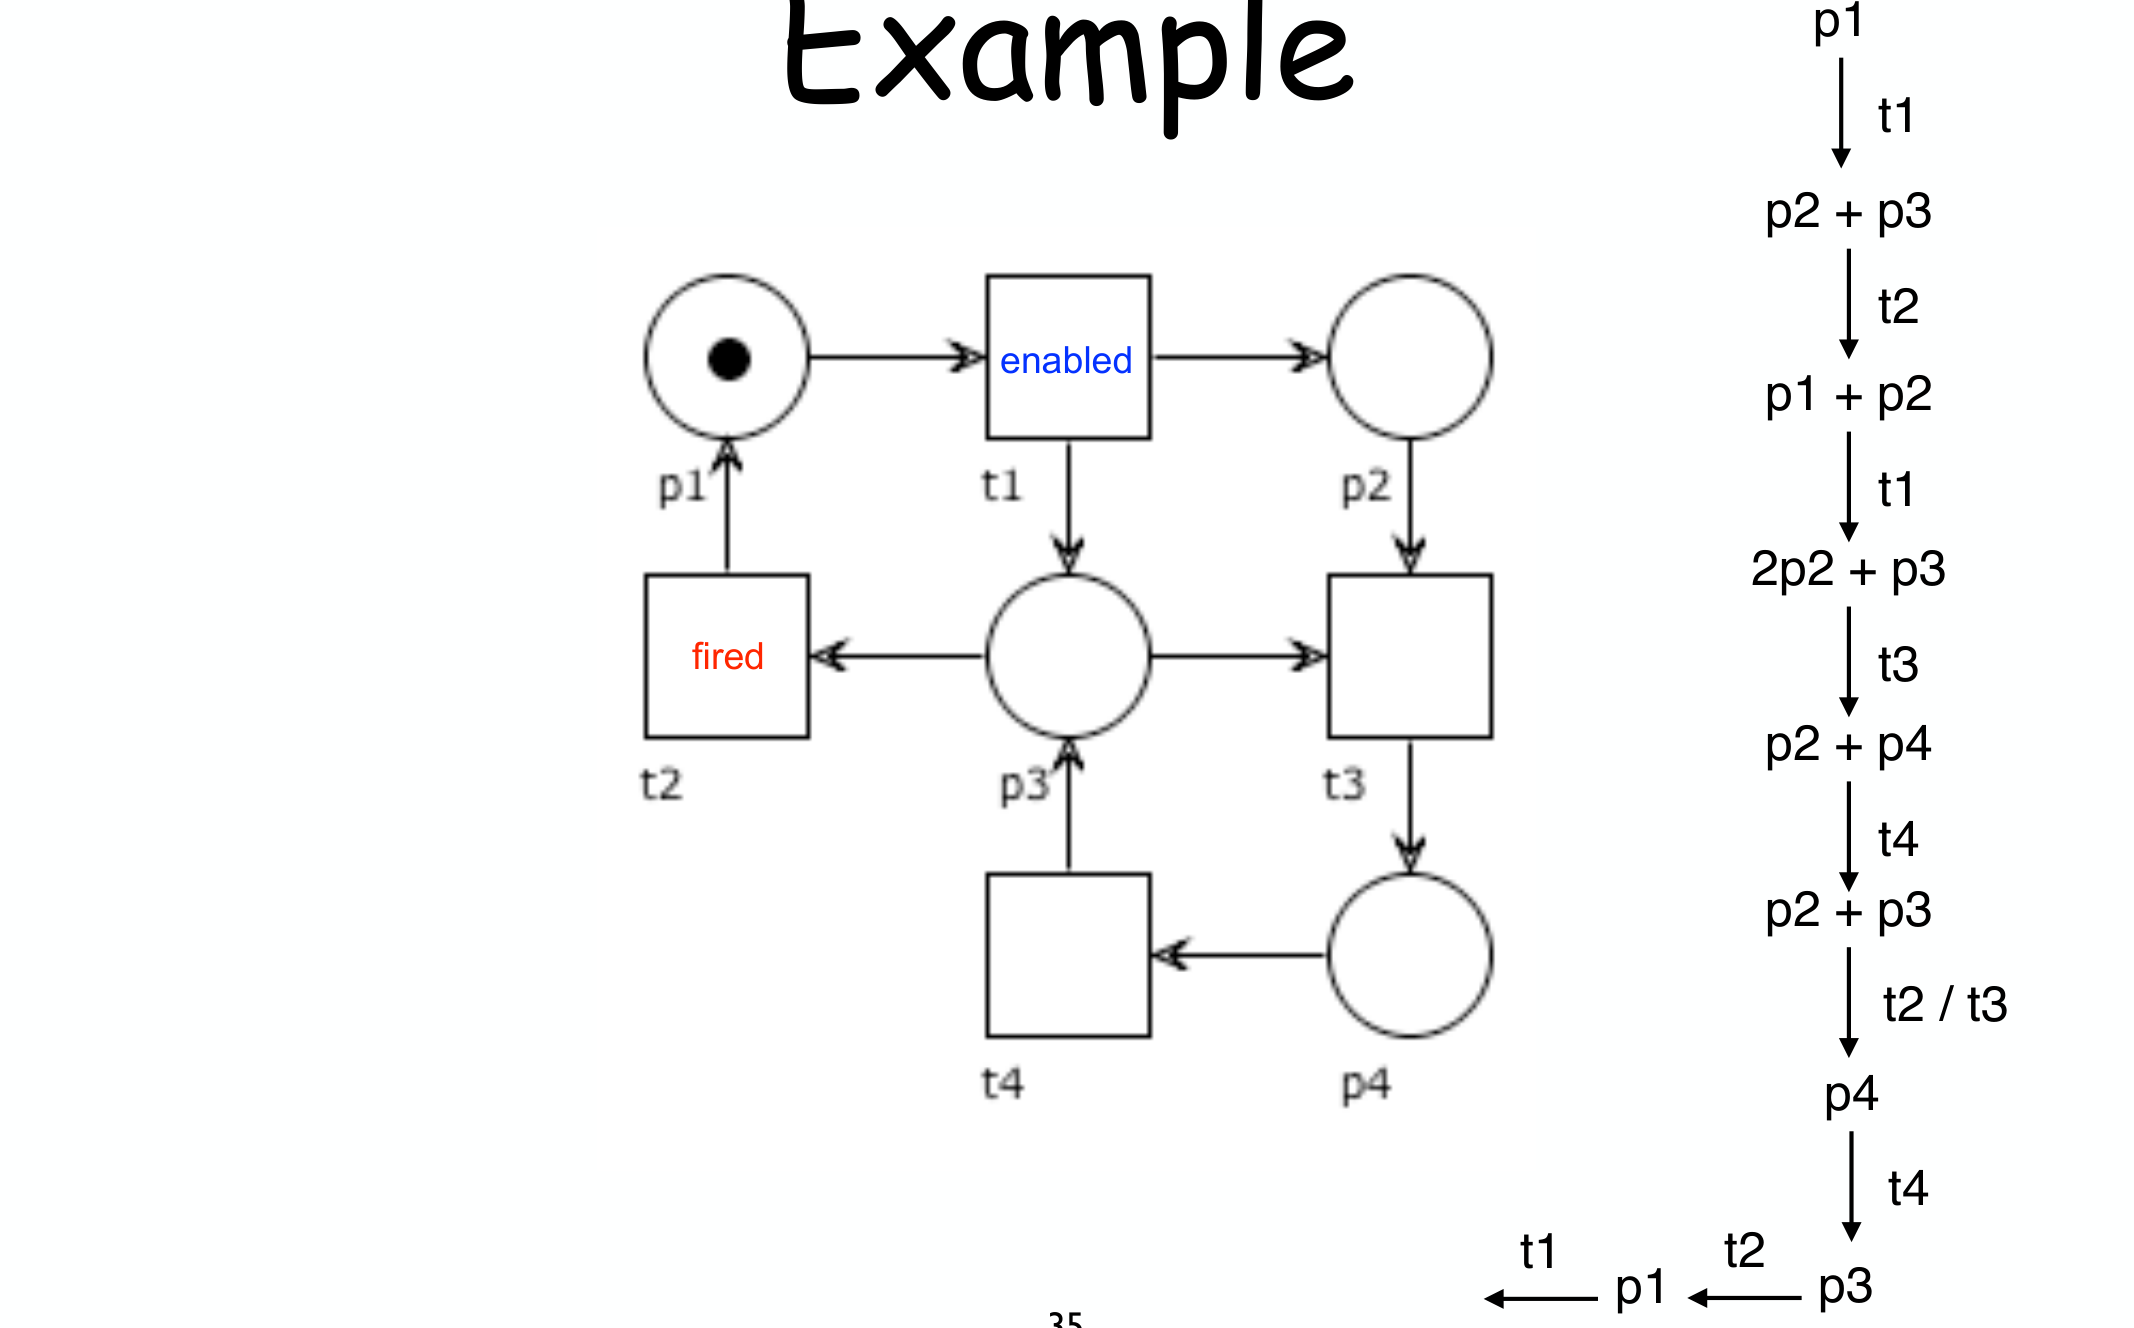
\includegraphics[width=0.74\linewidth,height=0.34\textheight,keepaspectratio]{images/04-petri_p34_token-game.png}
\caption{Token game. Una \textbf{marcatura} si scrive come somma formale dei token nei place: per esempio \texttt{2p2 + p3} significa due token in p2 e uno in p3. A ogni passo la transition abilitata (enabled) scatta (fired) e si passa alla marcatura successiva. Dove compaiono più transition abilitate insieme (\texttt{t2 / t3}) la scelta di quale far scattare è non-deterministica, e apre rami di evoluzione differenti.}
\end{figure}

\section{\texorpdfstring{Costruire i pattern di flusso con place e transition}{Costruire i pattern di flusso con place e transition}}

Il punto di forza dei Petri net, promesso all'inizio, è che i costrutti di control-flow (sequenza, parallelismo, scelta) \textbf{non richiedono simboli speciali}: nascono dal semplice modo in cui si dispongono place e transition. Vediamo come, ricordando la convenzione grafica: \textbf{cerchio = place, quadrato = transition, \textbullet\{\} = token}.

\textbf{Sequenza.} Per dire "$B$ dopo $A$" basta mettere un place tra le due transition: $A$ produce un token in quel place, che diventa la precondizione di $B$. L'ordine è forzato perché $B$ non può scattare finché $A$ non ha prodotto il suo token.

\begin{center}
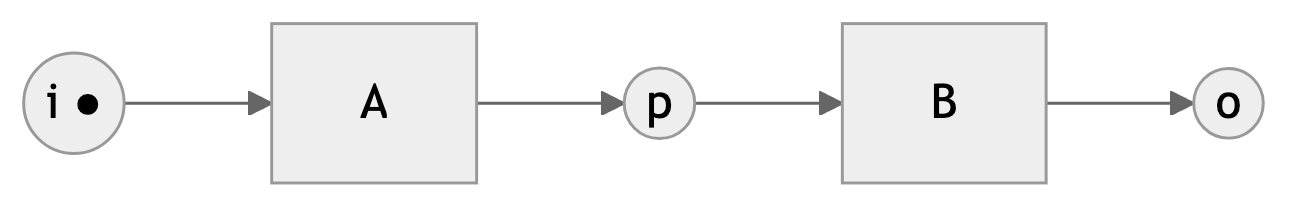
\includegraphics[width=0.74\linewidth,height=0.32\textheight,keepaspectratio]{images/mermaid/04_2.png}
\end{center}

\textbf{Parallelismo (AND-split e AND-join).} Se una \textbf{transition} ha \emph{più output place}, quando scatta mette un token in \emph{tutti} contemporaneamente: ha aperto più rami che procederanno in parallelo (AND-split). Simmetricamente, una transition con \emph{più input place} può scattare solo quando \emph{tutti} quei place hanno un token: aspetta il completamento di tutti i rami prima di proseguire (AND-join). Nell'esempio, $t1$ apre i due rami $p2$ e $p3$, e $t2$ li richiude aspettandoli entrambi.

\begin{center}
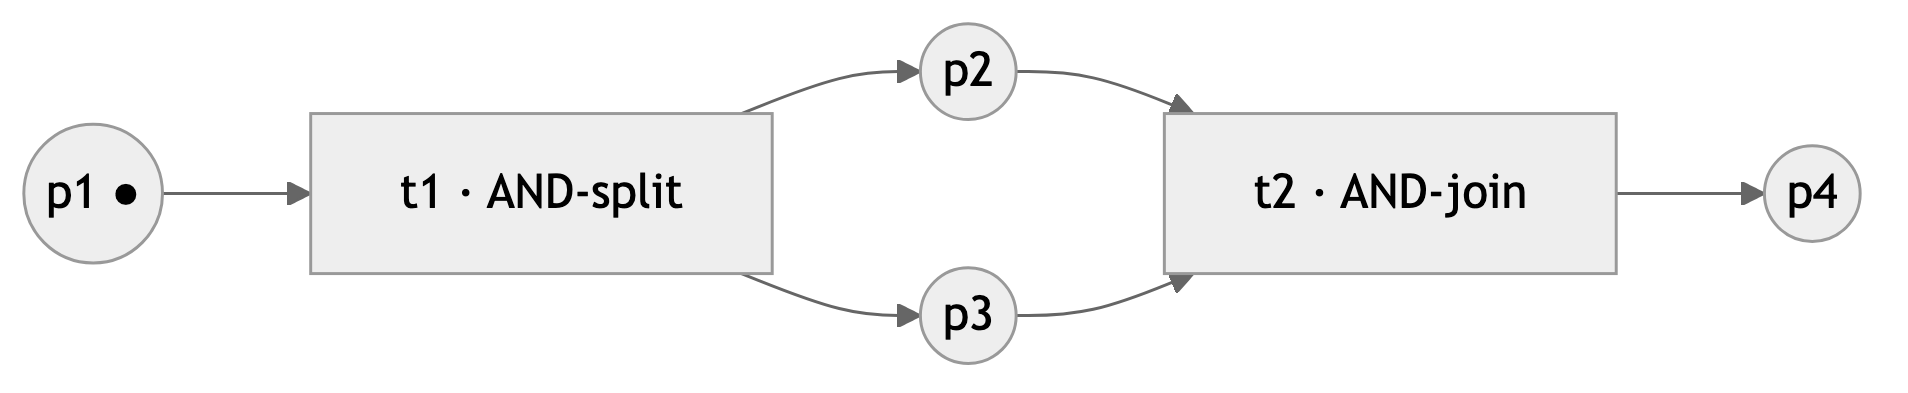
\includegraphics[width=0.74\linewidth,height=0.32\textheight,keepaspectratio]{images/mermaid/04_3.png}
\end{center}

\textbf{Scelta (XOR-split e XOR-join).} Qui è un \textbf{place} ad avere \emph{più transition uscenti}: il suo unico token può abilitare più transition, ma appena una scatta consuma il token e le altre non sono più abilitate. Si esegue quindi \emph{una sola} alternativa (XOR-split). Simmetricamente, un place con \emph{più transition entranti} raccoglie rami alternativi in un unico punto (XOR-join). Nell'esempio, dal place $p1$ si può eseguire $A$ \emph{oppure} $B$, ma non entrambi.

\begin{center}
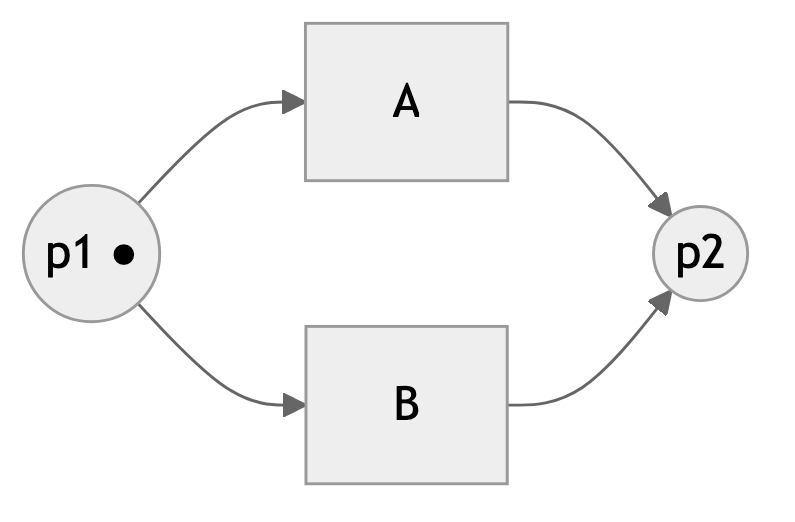
\includegraphics[width=0.49\linewidth,height=0.32\textheight,keepaspectratio]{images/mermaid/04_4.png}
\end{center}

\begin{boxtip}{La regola d'oro: guarda che tipo di nodo si dirama}
Tutta la differenza tra concorrenza e scelta sta in \textbf{quale nodo} si trova nel punto di diramazione: - se a diramarsi è una \textbf{transition} (un evento), i rami sono in \textbf{AND} $\rightarrow$ \emph{concorrenza}: tutti vengono attivati/attesi; - se a diramarsi è un \textbf{place} (una condizione con un token conteso), i rami sono in \textbf{XOR} $\rightarrow$ \emph{scelta}: solo uno vince il token.

Non serve nessun simbolo aggiuntivo: la semantica è già scritta nella struttura. È esattamente ciò che mancava ai gateway ambigui di \hyperref[ch:03]{03 — Visual Notation}.
\end{boxtip}

Esiste anche l'\textbf{OR-split} (attiva "uno o più" rami, non necessariamente tutti né esattamente uno), ma non è un costrutto elementare: si ottiene combinando AND e XOR, e lo tratteremo più avanti.

\section{\texorpdfstring{Workflow nets (WFN): Petri net su misura per i processi}{Workflow nets (WFN): Petri net su misura per i processi}}

I Petri net generici sono uno strumento potente ma \emph{troppo libero} per modellare un processo di business. Un processo ha caratteristiche precise che un Petri net qualsiasi non garantisce: comincia in un punto ben definito, finisce in un punto ben definito, e ogni sua parte deve avere un senso all'interno di quel percorso dall'inizio alla fine. I \textbf{workflow net} (WFN) sono Petri net a cui imponiamo esattamente queste restrizioni.

L'idea di fondo, prima ancora della definizione, è semplice: un processo ha un punto di \textbf{start}, dove entra un caso da lavorare; un blocco di \textbf{work}, cioè tutta la logica interna; e un punto di \textbf{end}, dove il caso esce concluso.

\begin{center}
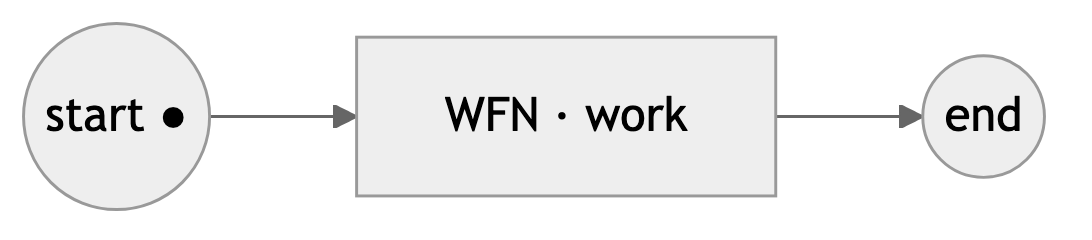
\includegraphics[width=0.67\linewidth,height=0.32\textheight,keepaspectratio]{images/mermaid/04_5.png}
\end{center}

\emph{Fig. — Un token nel place di start rappresenta un'istanza del processo non ancora avviata; quando quel token raggiunge il place di end, il caso è concluso.}

\begin{boxdefinition}{Workflow net}
Un Petri net $(P, T, F)$ è un \textbf{workflow net} se soddisfa tre condizioni:

\begin{enumerate}
\item esiste un place iniziale distinto $i \in P$ \textbf{senza archi entranti}:
\end{enumerate}

\begin{enumerate}
\item esiste un place finale distinto $o \in P$ \textbf{senza archi uscenti}:
\end{enumerate}

\begin{enumerate}
\item \textbf{ogni} altro place e transition si trova su almeno un \textbf{cammino da $i$ a $o$}.
\end{enumerate}
\end{boxdefinition}

Ognuna delle tre condizioni ha un significato concreto in termini di processo, che vale la pena esplicitare per capire \emph{perché} le imponiamo.

\begin{boxnote}{Perché proprio queste tre condizioni}
\begin{enumerate}
\item Un token nel place iniziale $i$ rappresenta \textbf{un'istanza del processo che è stata creata ma non ancora avviata}. Volere un unico $i$ significa volere un unico modo di "far entrare" un caso.
\item Un token nel place finale $o$ rappresenta \textbf{un caso ormai concluso}. Un unico $o$ significa un unico modo di "considerare finito" il processo.
\item Chiedere che ogni nodo stia su un cammino $i \to o$ significa vietare \textbf{parti inutili}: niente attività irraggiungibili dall'inizio, niente condizioni da cui non si esce mai. Ogni pezzo della rete deve poter partecipare all'elaborazione di almeno un caso.
\end{enumerate}
\end{boxnote}

Da queste condizioni segue una proprietà strutturale importante, che useremo spesso.

\begin{boxtheorem}{Unicità di source e sink}
In un workflow net, $i$ è \textbf{l'unico} nodo senza archi entranti e $o$ è \textbf{l'unico} nodo senza archi uscenti.

\emph{Dimostrazione (per $i$).} Supponiamo per assurdo che esista un altro nodo $v \neq i$ con $\bullet v = \varnothing$ (nessun arco entrante). Per la condizione 3, $v$ deve comparire in un cammino da $i$ a $o$. Ma un nodo senza archi entranti non può avere nulla che lo preceda in un cammino: potrebbe stare solo come \emph{primo} nodo del cammino. Il primo nodo di ogni cammino, però, è $i$. Quindi $v = i$, contro l'ipotesi. La dimostrazione per $o$ è del tutto analoga, scambiando "entrante" con "uscente" e "primo" con "ultimo". $\blacksquare$
\end{boxtheorem}

\begin{boxtip}{Come si riconosce (o si scarta) un workflow net}
In pratica, per stabilire se una rete è un WFN si controllano i tre requisiti. Le violazioni tipiche sono: - \textbf{manca un unico place iniziale}: ci sono più place senza archi entranti (più ingressi), oppure nessuno; - \textbf{c'è un nodo fuori da ogni cammino $i \to o$}: per esempio una transition $t$ che non è raggiungibile da $i$, oppure da cui non si arriva più a $o$ (un vicolo cieco).

Se invece l'ingresso e l'uscita sono unici e ogni nodo sta su un cammino da $i$ a $o$, allora la rete \textbf{è} un workflow net.
\end{boxtip}

\subsection{\texorpdfstring{Comporre processi: la strutturazione gerarchica}{Comporre processi: la strutturazione gerarchica}}

Avere un unico ingresso e un'unica uscita porta un vantaggio pratico enorme: permette di \textbf{comporre} i processi in modo gerarchico. Poiché un WFN, visto da fuori, si comporta come una scatola con un ingresso e un'uscita — esattamente come una singola transition — possiamo \textbf{raffinare una transition sostituendola con un intero workflow net}. Quella transition, che nel modello di alto livello era un'attività atomica, diventa così un \emph{sotto-processo} con la sua logica interna. Ripetendo il procedimento si costruiscono processi complessi per livelli successivi di dettaglio, tenendo ogni livello leggibile.

\section{\texorpdfstring{Syntax sugar: le decorazioni (e perché diffidarne)}{Syntax sugar: le decorazioni (e perché diffidarne)}}

Alcuni tool di modellazione, per far risparmiare spazio, permettono di "decorare" i punti di split e join con simboli sintetici (AND-split, AND-join, XOR-split, XOR-join) invece di disegnare per esteso la sotto-rete di place e transition. È \textbf{zucchero sintattico} (syntax sugar): una scorciatoia grafica che \emph{sta per} una struttura più estesa. Comodo, ma il professore mette in guardia con una nota personale esplicita.

\begin{figure}[!htb]
\centering
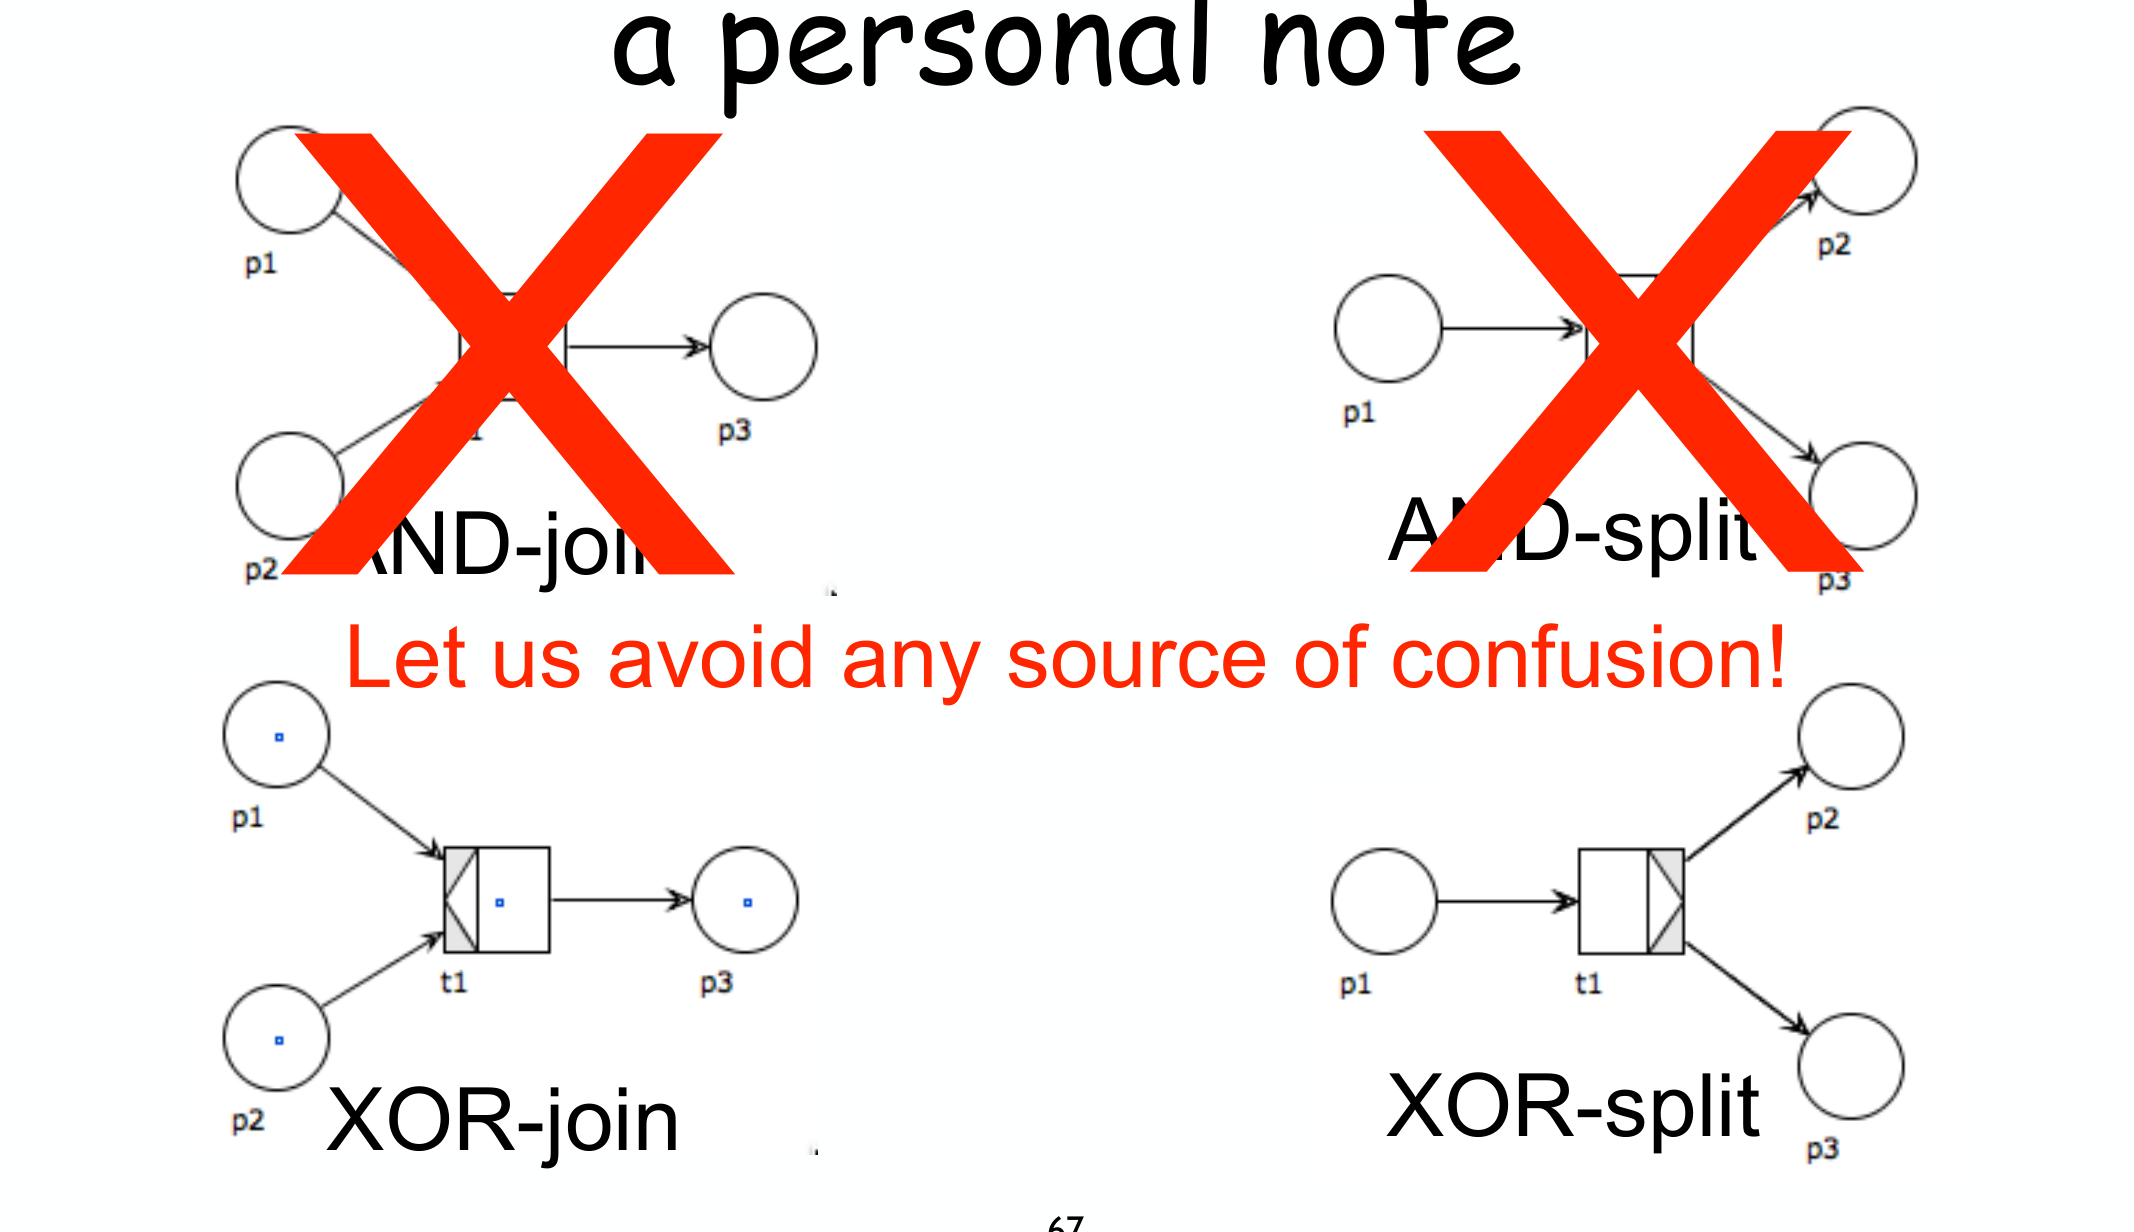
\includegraphics[width=0.74\linewidth,height=0.34\textheight,keepaspectratio]{images/04-petri_p66_sugar-note.png}
\caption{"Let us avoid any source of confusion!": le decorazioni di AND vengono barrate perché ridondanti, mentre quelle di XOR restano ma con l'avvertenza che vanno usate con cautela.}
\end{figure}

I problemi che rendono queste decorazioni infide sono tre, e conviene tenerli a mente perché toccano proprio la distinzione AND/XOR che abbiamo appena imparato a leggere dalla struttura:

\begin{boxwarning}{Perché le decorazioni ingannano}
\begin{itemize}
\item \textbf{Sono graficamente troppo simili}: i simboli di AND e di XOR si assomigliano, e confonderli significa scambiare la concorrenza con la scelta — un errore semantico grave.
\item \textbf{Cambiano significato a seconda di dove sono poste}: lo stesso simbolo posto su una transition o su un place vuol dire cose diverse (split contro join), quindi la posizione conta quanto il disegno.
\item \textbf{Per l'AND sono ridondanti}: la semantica AND è \emph{già} espressa dalla struttura (una transition che si dirama). Aggiungere una decorazione non porta informazione: appare solo per assomigliare ai gateway di BPMN. Meglio, allora, disegnare la rete esplicita e non lasciare spazio a fraintendimenti.
\end{itemize}
\end{boxwarning}

\section{\texorpdfstring{Il catalogo dei pattern di control-flow}{Il catalogo dei pattern di control-flow}}

Combinando i tre mattoni di base (sequenza, AND, XOR) si ottengono i pattern ricorrenti con cui si costruisce qualunque processo. Vale la pena averli a catalogo, con la loro "ricetta" in termini di split e join:

\begin{itemize}
\item \textbf{Sequencing} — $B$ è eseguito dopo $A$; è il place intermedio a imporre l'ordine.
\item \textbf{Parallelism} (AND-split + AND-join) — $A$ e $B$ vengono eseguiti \textbf{entrambi}, senza un ordine imposto tra loro; si aprono con un AND-split e si richiudono con un AND-join.
\item \textbf{Explicit choice} (XOR-split + XOR-join) — si esegue $A$ \textbf{oppure} $B$, e la scelta è \textbf{esplicita}, cioè risolta da una transition prima che i rami partano.
\item \textbf{Iteration} (XOR-join + XOR-split) — un ciclo: si ripete una porzione di processo \textbf{una o più volte} oppure \textbf{zero o più volte}, a seconda di dove si mettono join e split.
\item \textbf{Mutual exclusion} — $A$ e $B$ \textbf{non possono} eseguire in concorrenza perché condividono un token/una risorsa: chi lo prende esclude l'altro.
\item \textbf{Alternation} — $A$ e $B$ si eseguono \textbf{una volta ciascuno in alternanza} (prima $A$, poi $B$, poi di nuovo $A$...).
\end{itemize}

\subsection{\texorpdfstring{Scelta esplicita vs implicita (deferred): il concetto chiave}{Scelta esplicita vs implicita (deferred): il concetto chiave}}

Tra questi pattern ce n'è uno che merita attenzione particolare, perché tocca una domanda sottile: \textbf{chi} prende la decisione, e \textbf{quando}? La risposta distingue due tipi di scelta che sembrano uguali ma si comportano in modo diverso.

Nella \textbf{scelta esplicita}, esiste una transition il cui compito è proprio \emph{decidere}: scatta lei, e con il suo scatto instrada il processo su un ramo piuttosto che sull'altro. La decisione avviene \emph{dentro} il processo e \emph{prima} che i task alternativi diventino disponibili. In termini di token: la transition decisionale consuma il token e lo mette nel place del ramo scelto, così solo quel ramo risulta poi abilitato.

Nella \textbf{scelta implicita} (o \emph{deferred}, rimandata), invece, \textbf{nessuna transition decide}: sono i task alternativi stessi a competere. Tutti pescano dallo stesso place, quindi sono \textbf{abilitati insieme}; il primo che scatta consuma il token e taglia fuori gli altri. La decisione è quindi \emph{rimandata} al momento dello scatto ed è tipicamente determinata da un \textbf{evento esterno} (event-based): parte il task per cui l'evento arriva prima. La differenza pratica è netta e si vede nel diagramma.

\begin{figure}[!htb]
\centering
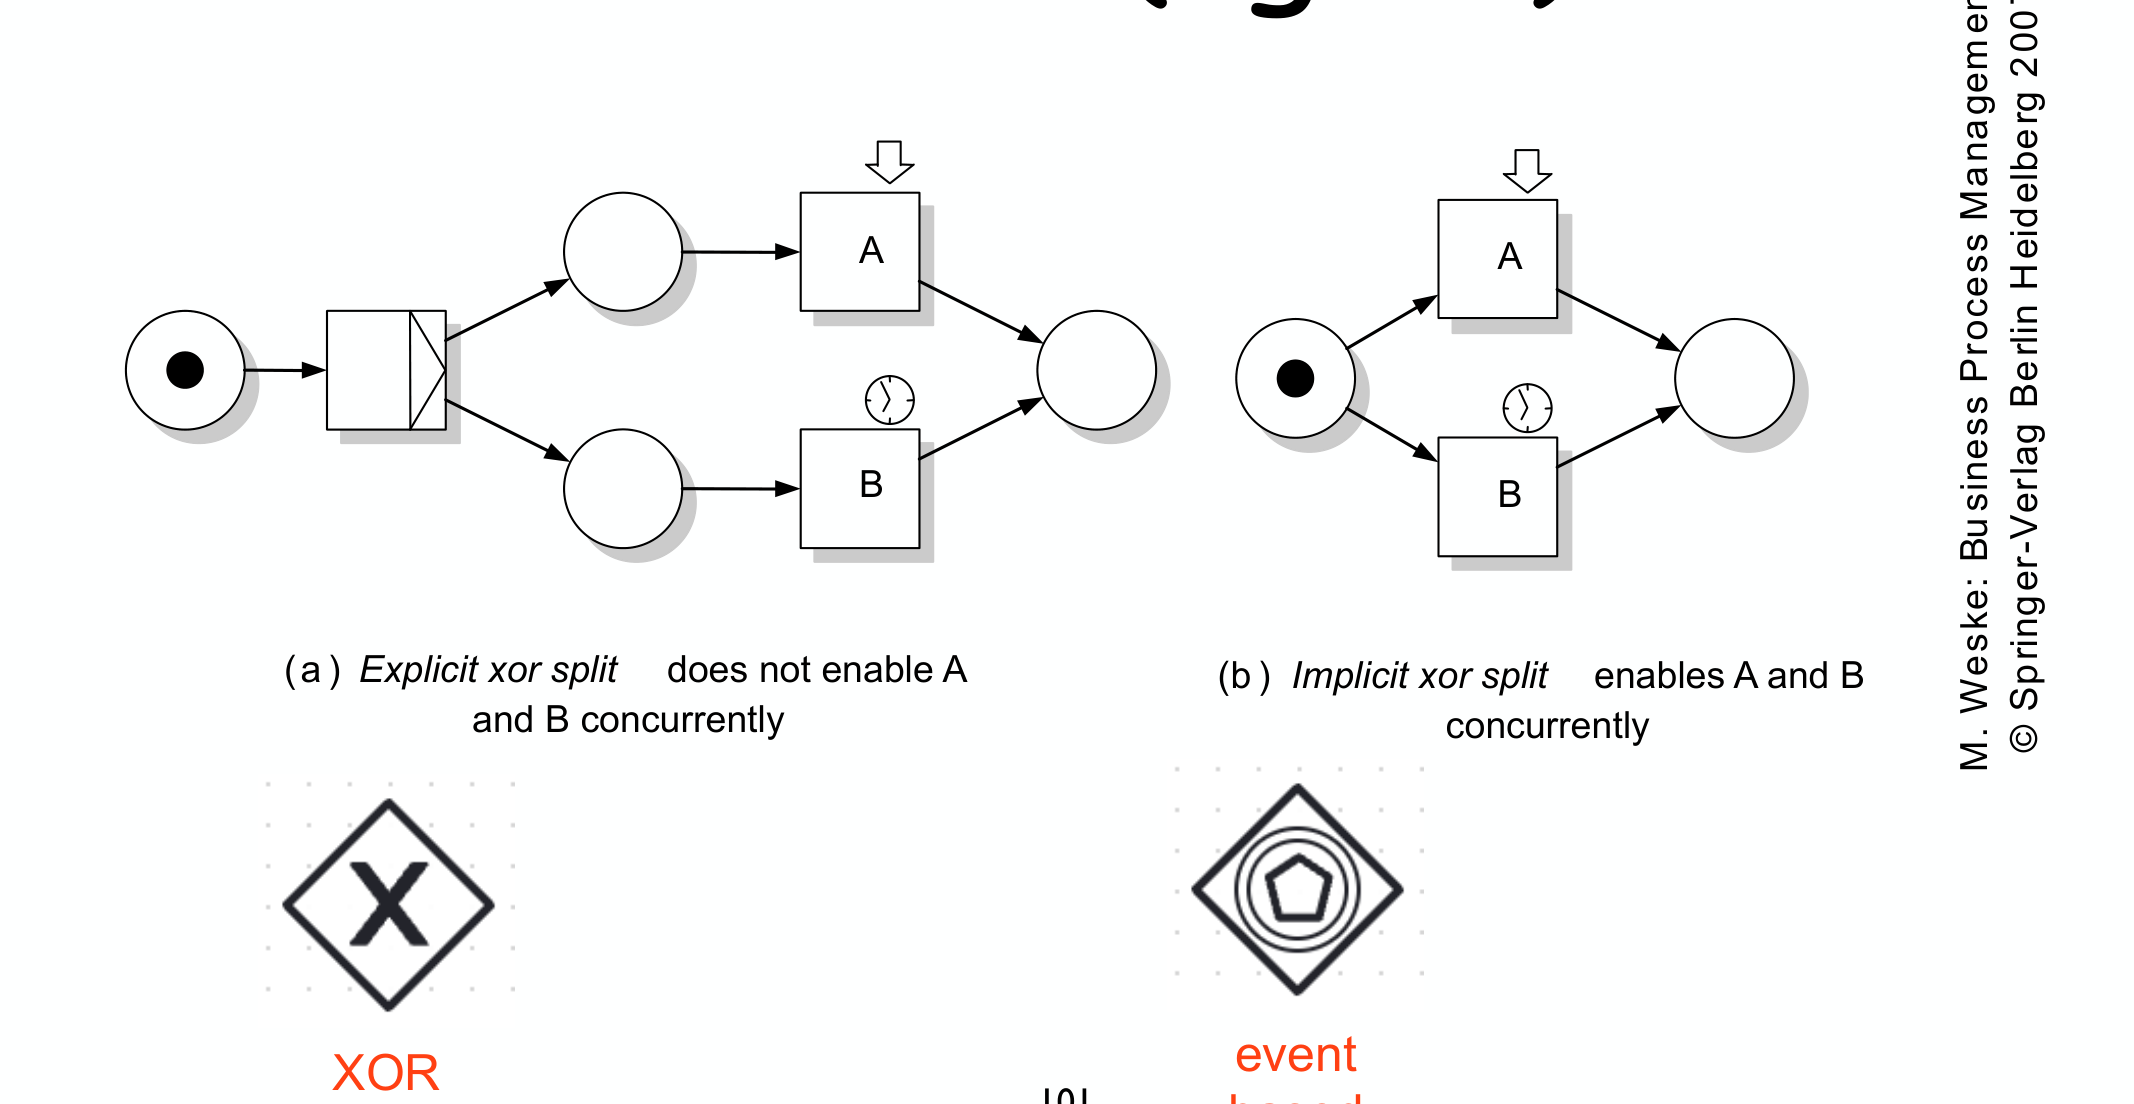
\includegraphics[width=0.74\linewidth,height=0.34\textheight,keepaspectratio]{images/04-petri_p100_explicit-vs-implicit.png}
\caption{(a) \textbf{Explicit}: c'è una transition-decisione (XOR) che sceglie il ramo; A e B non sono mai abilitati contemporaneamente. (b) \textbf{Implicit / deferred}: il token nel place iniziale abilita \textbf{sia} A \textbf{sia} B nello stesso momento, e vince chi scatta per primo (event-based; in BPMN corrisponde al gateway a pentagono). Nei due casi la decisione è presa in momenti diversi del tempo.}
\end{figure}

\section{\texorpdfstring{Trigger: chi fa scattare una transition}{Trigger: chi fa scattare una transition}}

Finora abbiamo descritto \emph{quando} una transition può scattare (regola di enabling), ma non \emph{chi} la fa scattare davvero. Nella realtà l'esecuzione dipende dall'\textbf{ambiente}: un'attività può partire da sola, oppure perché una persona la avvia, o perché arriva un messaggio, o perché scade un timer. I workflow net catturano questa informazione \textbf{decorando le transition con un trigger}, cioè annotando \emph{chi o cosa} è responsabile dello scatto di quel task.

\begin{figure}[!htb]
\centering
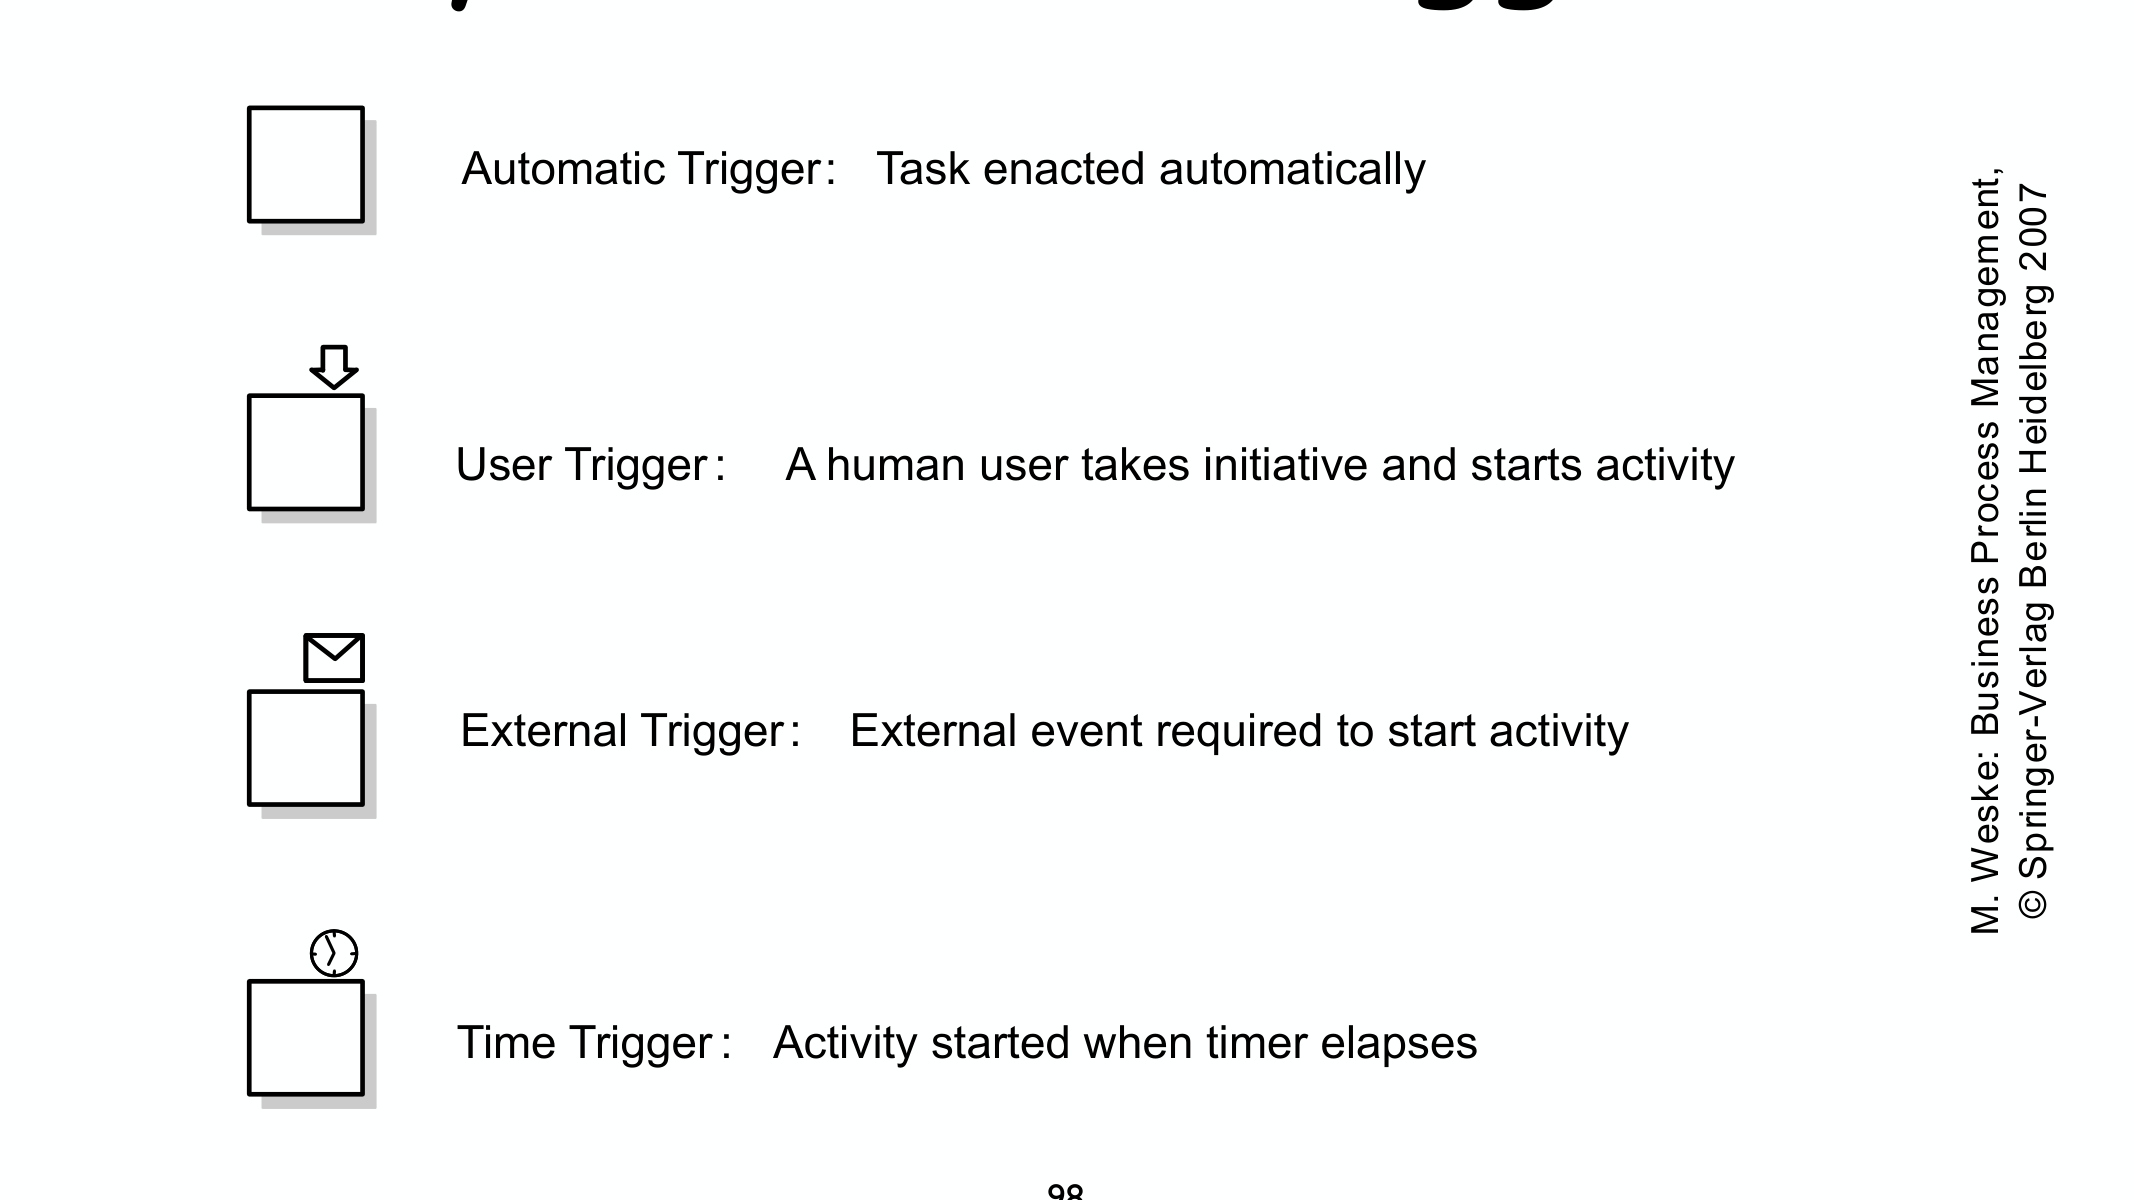
\includegraphics[width=0.74\linewidth,height=0.34\textheight,keepaspectratio]{images/04-petri_p97_triggers.png}
\caption{I simboli dei trigger (Weske).}
\end{figure}

\begin{boxdefinition}{I quattro tipi di trigger}
\begin{itemize}
\item \textbf{Automatic trigger} (nessun simbolo): il task scatta \textbf{automaticamente} non appena è abilitato, senza bisogno di alcun intervento. È il caso di default.
\item \textbf{User trigger} (una freccia): serve l'\textbf{iniziativa di una persona}, che decide di avviare l'attività.
\item \textbf{External trigger} (una busta): serve un \textbf{evento esterno}, tipicamente la ricezione di un messaggio, perché l'attività parta.
\item \textbf{Time trigger} (un orologio): l'attività parte allo \textbf{scadere di un timer} (per esempio un time-out).
\end{itemize}

Le transition prive di trigger sono, per convenzione, automatiche.
\end{boxdefinition}

I trigger sono anche il legame naturale con la scelta implicita vista sopra: quando più task in \emph{deferred choice} aspettano ciascuno un evento esterno diverso, è il primo trigger a scattare che risolve la competizione.

Con Petri net, workflow net, token game e la distinzione tra scelta esplicita e implicita abbiamo la \textbf{base formale} del corso. Su di essa costruiremo, nelle prossime lezioni, gli strumenti di analisi dei processi: raggiungibilità degli stati, liveness, soundness. $\rightarrow$ \hyperref[ch:05]{05 — Mining}